\documentclass[8pt]{beamer}
    \usepackage{graphicx}
    \usepackage{wrapfig}
    \usepackage{multicol}

    \usepackage[T1]{fontenc}
    \usepackage{mathptmx}
    \usetheme{Madrid}
    
    \title{Wicked Witch - ANOVA}
    \author{Ahmed Ayman}
    
    \begin{document}
        \maketitle
        \begin{frame}{Agenda}
            \begin{itemize}
                \item The story
                \item Dataset
                \item Business and Statistical Question
                \item Assumption checks
                \item test result
                \item after statistical significant difference
            \end{itemize}
        \end{frame}

        \begin{frame}{The story}
            A wicked witch make troubles in different areas [east, west, north, and south]\\
            \textbf{investigation team wonder if she makes troubles in some ares more than other areas}\\
            \begin{columns}
                \column{.5\textwidth}
                \centering
                
\includegraphics[height=.75\textheight]{images/wicked-old-witch.jpg}
                \column{.5\textwidth}
                \centering
                
\includegraphics[width=.95\textwidth]{images/investigator.jpg}
            \end{columns}
        \end{frame}

        \begin{frame}{Dataset}
            Our Data contains two columns
            \begin{itemize}
                \item \textbf{Area:} an ordinal variable indicates the area
                \item \textbf{Complains:} a scaler variable indicates number of Complains we received from the citizens
            \end{itemize}
            \centering
            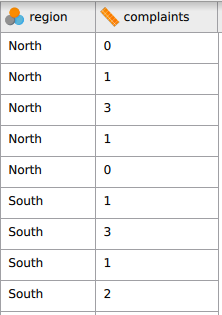
\includegraphics[height=.5\textheight]{images/data.png}
        \end{frame}

        \begin{frame}{Business and Statistical Question}
            \begin{block}{\textbf{Questions}}
                \begin{itemize}
                    \item \textbf{Business:} Does she make troubles in some ares more than other areas?!
                    \item \textbf{Statistical:} Complains(Area 1) = Complains(Area 2) \ldots = Complains(Area n)
                \end{itemize}
            \end{block}

            \begin{block}{\textbf{The test}}
                The Statistical test is \textcolor{red}{\textbf{ANOVA}} (Hope: this test to be statistically significant)\\
                This test requires some assumptions check \\ 
                \begin{itemize}
                    \item Equality fo variance 
                    \item We hope those tests to be \textbf{(statistically not significant)}
                \end{itemize}
            \end{block}
        \end{frame}

        \begin{frame}{Assumption checks}
            \begin{columns}
                \column{.45\textwidth}
                \begin{itemize}
                    \item The p-value of \textbf{Levene-test} < .05
                    \item which means: The groups have similar variance: \textcolor{blue}{\textbf{Great}}
                \end{itemize}
                \column{.55\textwidth}
                \begin{figure}
                    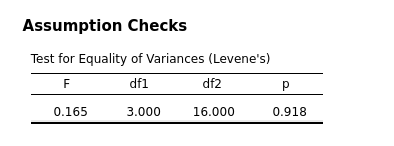
\includegraphics[width=.95\textwidth]{images/ANOVA assumptions.png}
                    \vspace{.25cm}
                \end{figure}
            \end{columns}
        \end{frame}

        \begin{frame}{test result}
            \begin{columns}
                \column{.45\textwidth}
                \begin{itemize}
                    \item The p-value is much less than .05
                    \item Which means there is difference in wicked witch behavior from area to another
                    \item also the \textbf{Effect size} is large
                    \item So, we confidently reject the $H_0$
                    \item \textcolor{blue}{\textbf{Great}}
                \end{itemize}
                \column{.55\textwidth}
                \begin{figure}
                    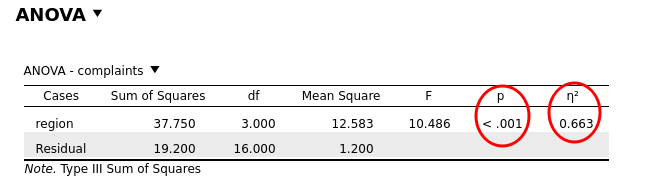
\includegraphics[width=.95\textwidth]{images/ANOVA result.png}
                    \vspace{.25cm}
                \end{figure}
            \end{columns}
        \end{frame}

        \begin{frame}{after statistical significant difference}
            As we are all know ANOVA is an omnibus test, which tells us if there is a difference between groups or not.\\
            But don't tell us, which group is different, to know we have to do more analysis.\\
            \begin{columns}
                \column{.55\textwidth}
                From the Post Hoc, and the visualization we see:
                \begin{itemize}
                    \item east and west contain more complains than other area
                    \item west contains highest number of complains.
                \end{itemize}
                \column{.45\textwidth}
                \centering
                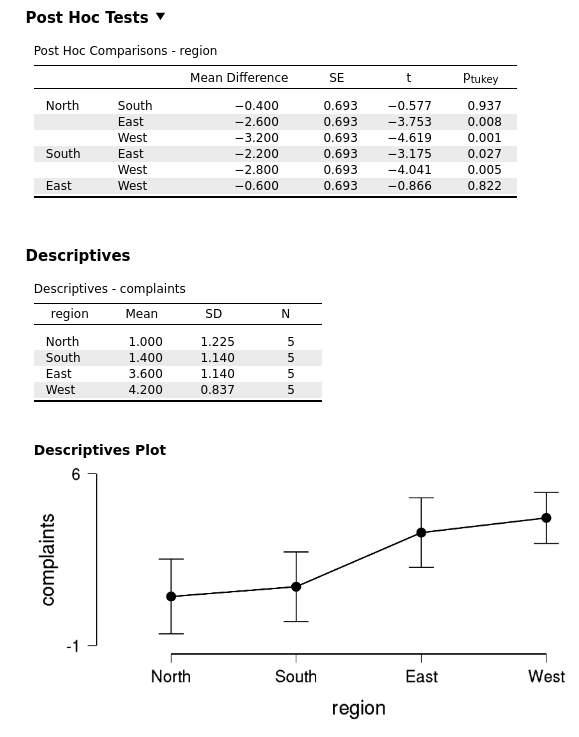
\includegraphics[width=.95\textwidth]{images/after ANOVA.png}
            \end{columns}
        \end{frame}
    \end{document}